% Detailed GauCon Head Module Architecture (English, CVPR/WACV style — relative positioning)
\documentclass[tikz,border=3pt]{standalone}
\usepackage{fontspec}
\usepackage{amsmath,amssymb}
\setmainfont{DejaVu Serif}
\usetikzlibrary{positioning,fit,calc,arrows.meta,backgrounds}

\definecolor{cInk}{HTML}{1F2937}
\definecolor{cIn}{HTML}{F1F5F9}
\definecolor{cGeo}{HTML}{FFF3E0}
\definecolor{cGeoB}{HTML}{C2410C}
\definecolor{cBox}{HTML}{FEE2E2}
\definecolor{cBoxB}{HTML}{B91C1C}
\definecolor{cCls}{HTML}{D1FAE5}
\definecolor{cClsB}{HTML}{047857}
\definecolor{cPar}{HTML}{E0F2FE}

\begin{document}
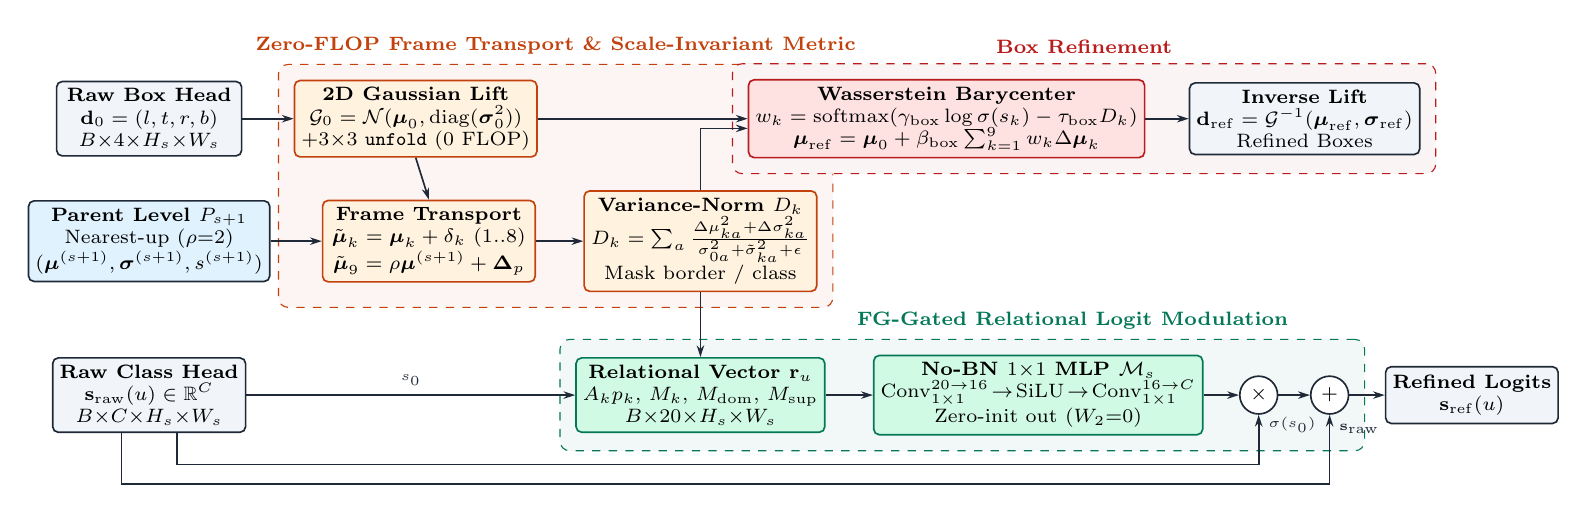
\begin{tikzpicture}[
  font=\scriptsize,
  blk/.style={draw=cInk, fill=#1, semithick, rounded corners=2pt,
              align=center, inner sep=2.5pt, minimum height=7.2mm},
  op/.style={circle, draw=cInk, fill=white, semithick, inner sep=0pt, minimum size=4.8mm, font=\scriptsize\bfseries},
  arr/.style={-{Stealth[length=1.5mm,width=0.95mm]}, cInk, semithick},
  zone/.style={draw=#1, dashed, rounded corners=3.5pt, fill=#1!5!white, inner sep=5.5pt},
]

% Stage 1 (Vertical Stack Left)
\node[blk=cIn, minimum width=2.35cm] (raw_box)
  {\textbf{Raw Box Head}\\$\mathbf{d}_0 = (l, t, r, b)$\\$B{\times}4{\times}H_s{\times}W_s$};
\node[blk=cPar, minimum width=2.35cm, below=0.55cm of raw_box] (par_in)
  {\textbf{Parent Level $P_{s+1}$}\\Nearest-up ($\rho{=}2$)\\$(\boldsymbol{\mu}^{(s+1)},\boldsymbol{\sigma}^{(s+1)}, s^{(s+1)})$};
\node[blk=cIn, minimum width=2.35cm, below=0.95cm of par_in] (raw_cls)
  {\textbf{Raw Class Head}\\$\mathbf{s}_{\mathrm{raw}}(u) \in \mathbb{R}^C$\\$B{\times}C{\times}H_s{\times}W_s$};

% Stage 2 (Transport & Scale-Invariant Metric)
\node[blk=cGeo, draw=cGeoB, minimum width=2.70cm, right=0.65cm of raw_box] (lift)
  {\textbf{2D Gaussian Lift}\\$\mathcal{G}_0=\mathcal{N}(\boldsymbol{\mu}_0,\mathrm{diag}(\boldsymbol{\sigma}_0^2))$\\$+3{\times}3$ \texttt{unfold} ($0$ FLOP)};
\node[blk=cGeo, draw=cGeoB, minimum width=2.70cm, right=0.65cm of par_in] (trans)
  {\textbf{Frame Transport}\\$\tilde{\boldsymbol{\mu}}_k = \boldsymbol{\mu}_k + \delta_k$ ($1..8$)\\$\tilde{\boldsymbol{\mu}}_9 = \rho\boldsymbol{\mu}^{(s+1)}+\boldsymbol{\Delta}_p$};
\node[blk=cGeo, draw=cGeoB, minimum width=2.75cm, right=0.60cm of trans] (metric)
  {\textbf{Variance-Norm $D_k$}\\$D_k = \sum_{a}\frac{\Delta\mu_{ka}^2+\Delta\sigma_{ka}^2}{\sigma_{0a}^2+\tilde{\sigma}_{ka}^2+\epsilon}$\\Mask border / class};

% Stage 3a (Regression Barycenter Branch — Top Row)
\node[blk=cBox, draw=cBoxB, minimum width=3.55cm, right=0.60cm of metric |- lift] (bary)
  {\textbf{Wasserstein Barycenter}\\$w_k = \mathrm{softmax}(\gamma_{\mathrm{box}}\log\sigma(s_k)-\tau_{\mathrm{box}}D_k)$\\$\boldsymbol{\mu}_{\mathrm{ref}}=\boldsymbol{\mu}_0+\beta_{\mathrm{box}}\sum_{k=1}^9 w_k\Delta\boldsymbol{\mu}_k$};
\node[blk=cIn, minimum width=2.05cm, right=0.55cm of bary] (inv)
  {\textbf{Inverse Lift}\\$\mathbf{d}_{\mathrm{ref}}=\mathcal{G}^{-1}(\boldsymbol{\mu}_{\mathrm{ref}},\boldsymbol{\sigma}_{\mathrm{ref}})$\\Refined Boxes};

% Stage 3b (Classification Relational Gate — Bottom Row, spaced cleanly below metric)
\node[blk=cCls, draw=cClsB, minimum width=2.75cm] at (metric |- raw_cls) (rel)
  {\textbf{Relational Vector $\mathbf{r}_u$}\\$A_k p_k$, $M_k$, $M_{\mathrm{dom}}$, $M_{\mathrm{sup}}$\\$B{\times}20{\times}H_s{\times}W_s$};
\node[blk=cCls, draw=cClsB, minimum width=3.55cm, right=0.60cm of rel] (mlp)
  {\textbf{No-BN $1{\times}1$ MLP $\mathcal{M}_s$}\\$\mathrm{Conv}_{1\times 1}^{20\to 16}\!\to\!\mathrm{SiLU}\!\to\!\mathrm{Conv}_{1\times 1}^{16\to C}$\\Zero-init out ($W_2{=}0$)};

\node[op, right=0.45cm of mlp] (mul) {$\times$};
\node[op, right=0.40cm of mul] (add) {$+$};
\node[blk=cIn, minimum width=1.80cm, right=0.45cm of add] (clsout)
  {\textbf{Refined Logits}\\$\mathbf{s}_{\mathrm{ref}}(u)$};

% Clean Orthogonal Routing
\draw[arr] (raw_box.east) -- (lift.west);
\draw[arr] (lift.south) -- (trans.north);
\draw[arr] (par_in.east) -- (trans.west);
\draw[arr] (trans.east) -- (metric.west);

\draw[arr] (lift.east) -- (bary.west);
\draw[arr] (metric.north) |- ([yshift=-3.5pt]bary.west);
\draw[arr] (bary.east) -- (inv.west);

\draw[arr] (metric.south) -- (rel.north);
\draw[arr] (raw_cls.east) -- node[above, font=\tiny]{$s_0$} (rel.west);
\draw[arr] (rel.east) -- (mlp.west);
\draw[arr] (mlp.east) -- (mul.west);
\draw[arr] (mul.east) -- (add.west);
\draw[arr] (add.east) -- (clsout.west);

\draw[arr] ([xshift=0.35cm]raw_cls.south) -- ++(0,-0.40) -| node[pos=0.90, right, font=\tiny]{$\sigma(s_0)$} (mul.south);
\draw[arr] ([xshift=-0.35cm]raw_cls.south) -- ++(0,-0.65) -| node[pos=0.90, right, font=\tiny]{$\mathbf{s}_{\mathrm{raw}}$} (add.south);

\begin{scope}[on background layer]
  \node[zone=cGeoB, fit=(lift)(trans)(metric), label={[font=\scriptsize\bfseries, text=cGeoB]above:{Zero-FLOP Frame Transport \& Scale-Invariant Metric}}] {};
  \node[zone=cBoxB, fit=(bary)(inv), label={[font=\scriptsize\bfseries, text=cBoxB]above:{Box Refinement}}] {};
  \node[zone=cClsB, fit=(rel)(mlp)(mul)(add), label={[font=\scriptsize\bfseries, text=cClsB, xshift=1.4cm]above:{FG-Gated Relational Logit Modulation}}] {};
\end{scope}

\end{tikzpicture}
\end{document}
